\clearpage
\phantomsection

\addcontentsline{toc}{chapter}{{PHỤ LỤC}}
\chapter*{Phụ lục}
\renewcommand{\thefigure}{A.\arabic{figure}} 
\setcounter{figure}{0}
\begin{enumerate}[A$).$]

	% \item {Flow-graph mô phỏng DOA với dữ liệu Matlab trên GNU Radio.
	% 		\par
	% 		\begin{figure} [!h]
	% 		\centering
	% 		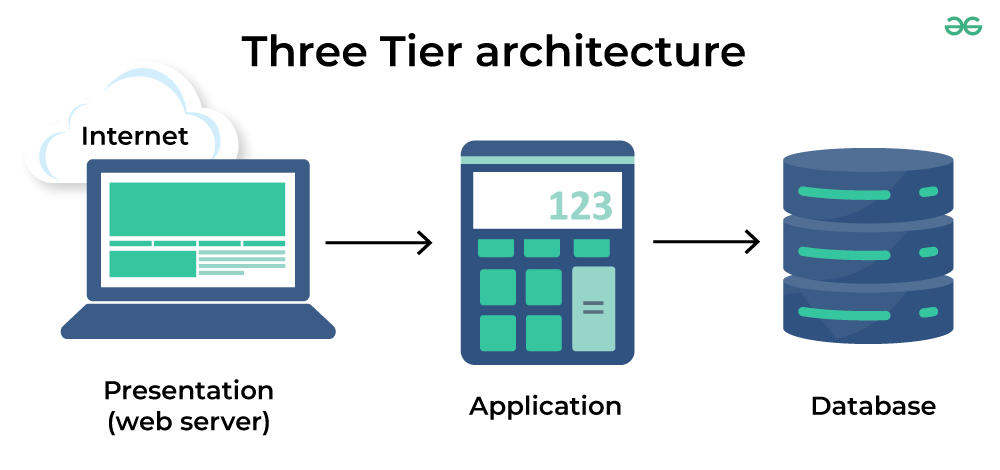
\includegraphics[width=1\linewidth]{figures/three-tier-architecture.png}
	% 		\caption{Flow-graph ước lượng DOA với dữ liệu mô phỏng Matlab trên GNU Radio}
	% 		\label{fig:simulation1}
	% 		\end{figure} 
	% 		\newpage}
	% \item {
	% 	Mô phỏng dữ liệu thu từ BladeRF, vừa chịu ảnh hưởng từ kênh truyền, vừa chịu ảnh hưởng do sai số phần cứng BladeRF gây ra.
	% 	\renewcommand{\thefigure}{B.\arabic{figure}} 
	% 	\setcounter{figure}{0}
	% 	 \begin{figure}[!ht]
	% 		%\hfill
	% 		\centering
	% 		\subfigure[Mô phỏng tạp âm và nhiễu đa đường]{\includegraphics[width=1\linewidth]{figures/channel.png}
	% 			\label{fig:channel}}
	% 		\hfill
	% 		\subfigure[Mô phỏng $\textrm{sample}_\textrm{offset}$ và $\textrm{phase}_\textrm{offset}$]{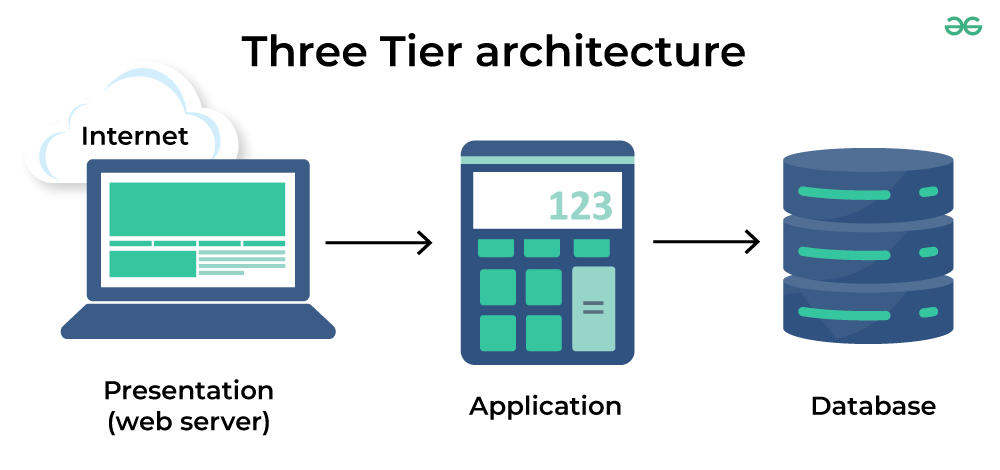
\includegraphics[width=0.5\linewidth]{figures/three-tier-architecture.png}\label{fig:sampleandphase}}
	% 		\hfill
	% 		\caption{Mô phỏng dữ liệu BladeRF qua kênh truyền}
	% 		\label{fig:bladesimu}
	% 	\end{figure}
	% \newpage
	% }

	
% 	\item {
% 		Flow-graph điều chế tín hiệu truyền hình chuẩn DVB-T trên GNU Radio.
% 	\renewcommand{\thefigure}{E.\arabic{figure}} 
% 	\setcounter{figure}{0}
% 	\begin{figure} [!h]
% 		\centering
% 		\includegraphics[width=0.95\linewidth]{figures/dvbt.png}
% 		\caption{Flow-graph truyền tín hiệu DVB-T}
% 		\label{fig:dvbt}
% 	\end{figure}	
% }
\end{enumerate}